\documentclass{standalone}
\usepackage{tikz}
\usetikzlibrary{patterns, positioning}


\begin{document}
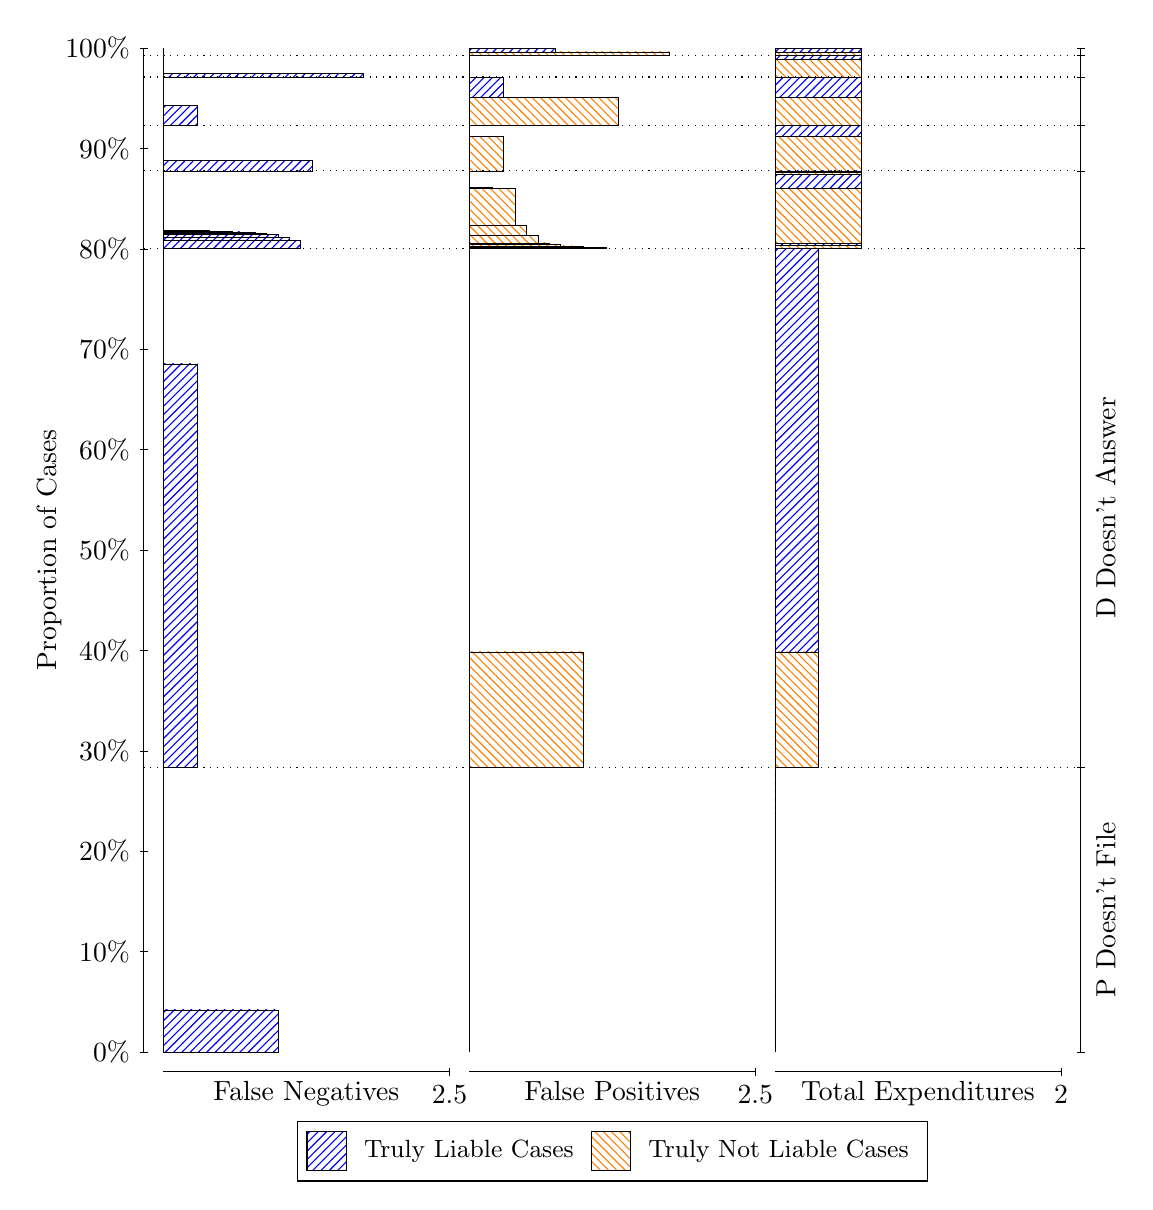
\begin{tikzpicture}
\draw[black, very thin] (1.5,1.75) -- (1.5,14.5);
\node[rotate=90, text=black, anchor=center] at (0.3, 8.125) {Proportion of Cases};
\draw[black, very thin] (1.45,1.75) -- (1.55,1.75);
\node[text=black, anchor=east] at (1.45, 1.75) {0\%};
\draw[black, very thin] (1.45,3.025) -- (1.55,3.025);
\node[text=black, anchor=east] at (1.45, 3.025) {10\%};
\draw[black, very thin] (1.45,4.3) -- (1.55,4.3);
\node[text=black, anchor=east] at (1.45, 4.3) {20\%};
\draw[black, very thin] (1.45,5.575) -- (1.55,5.575);
\node[text=black, anchor=east] at (1.45, 5.575) {30\%};
\draw[black, very thin] (1.45,6.85) -- (1.55,6.85);
\node[text=black, anchor=east] at (1.45, 6.85) {40\%};
\draw[black, very thin] (1.45,8.125) -- (1.55,8.125);
\node[text=black, anchor=east] at (1.45, 8.125) {50\%};
\draw[black, very thin] (1.45,9.4) -- (1.55,9.4);
\node[text=black, anchor=east] at (1.45, 9.4) {60\%};
\draw[black, very thin] (1.45,10.675) -- (1.55,10.675);
\node[text=black, anchor=east] at (1.45, 10.675) {70\%};
\draw[black, very thin] (1.45,11.95) -- (1.55,11.95);
\node[text=black, anchor=east] at (1.45, 11.95) {80\%};
\draw[black, very thin] (1.45,13.225) -- (1.55,13.225);
\node[text=black, anchor=east] at (1.45, 13.225) {90\%};
\draw[black, very thin] (1.45,14.5) -- (1.55,14.5);
\node[text=black, anchor=east] at (1.45, 14.5) {100\%};

\draw[black, very thin] (13.4,1.75) -- (13.4,14.5);
\draw[black, very thin] (13.35,1.75) -- (13.45,1.75);
\node[anchor=west] at (13.35, 1.75) {};
\draw[black, very thin] (13.35,5.3604) -- (13.45,5.3604);
\node[anchor=west] at (13.35, 5.3604) {};
\draw[black, very thin] (13.35,11.959) -- (13.45,11.959);
\node[anchor=west] at (13.35, 11.959) {};
\draw[black, very thin] (13.35,12.941) -- (13.45,12.941);
\node[anchor=west] at (13.35, 12.941) {};
\draw[black, very thin] (13.35,13.513) -- (13.45,13.513);
\node[anchor=west] at (13.35, 13.513) {};
\draw[black, very thin] (13.35,14.132) -- (13.45,14.132);
\node[anchor=west] at (13.35, 14.132) {};
\draw[black, very thin] (13.35,14.405) -- (13.45,14.405);
\node[anchor=west] at (13.35, 14.405) {};
\draw[black, very thin] (13.35,14.5) -- (13.45,14.5);
\node[anchor=west] at (13.35, 14.5) {};

\draw[black, very thin, pattern color=blue, pattern=north east lines] (1.75,1.75) rectangle (3.2033,2.2853);
\draw[black, very thin, pattern color=orange, pattern=north west lines] (1.75,2.2853) rectangle (1.75,5.3604);
\draw[black, very thin, pattern color=blue, pattern=north east lines] (1.75,5.3604) rectangle (2.186,10.489);
\draw[black, very thin, pattern color=orange, pattern=north west lines] (1.75,10.489) rectangle (1.75,11.959);
\draw[black, very thin, pattern color=blue, pattern=north east lines] (1.75,11.959) rectangle (3.494,12.055);
\draw[black, very thin, pattern color=blue, pattern=north east lines] (1.75,12.055) rectangle (3.3487,12.095);
\draw[black, very thin, pattern color=blue, pattern=north east lines] (1.75,12.095) rectangle (3.2033,12.136);
\draw[black, very thin, pattern color=blue, pattern=north east lines] (1.75,12.136) rectangle (3.058,12.139);
\draw[black, very thin, pattern color=blue, pattern=north east lines] (1.75,12.139) rectangle (3.058,12.145);
\draw[black, very thin, pattern color=blue, pattern=north east lines] (1.75,12.145) rectangle (2.9127,12.158);
\draw[black, very thin, pattern color=blue, pattern=north east lines] (1.75,12.158) rectangle (2.7673,12.164);
\draw[black, very thin, pattern color=blue, pattern=north east lines] (1.75,12.164) rectangle (2.622,12.171);
\draw[black, very thin, pattern color=blue, pattern=north east lines] (1.75,12.171) rectangle (2.4767,12.174);
\draw[black, very thin, pattern color=blue, pattern=north east lines] (1.75,12.174) rectangle (2.3313,12.182);
\draw[black, very thin, pattern color=orange, pattern=north west lines] (1.75,12.182) rectangle (1.75,12.941);
\draw[black, very thin, pattern color=blue, pattern=north east lines] (1.75,12.941) rectangle (3.6393,13.075);
\draw[black, very thin, pattern color=orange, pattern=north west lines] (1.75,13.075) rectangle (1.75,13.513);
\draw[black, very thin, pattern color=blue, pattern=north east lines] (1.75,13.513) rectangle (2.186,13.771);
\draw[black, very thin, pattern color=orange, pattern=north west lines] (1.75,13.771) rectangle (1.75,14.132);
\draw[black, very thin, pattern color=blue, pattern=north east lines] (1.75,14.132) rectangle (4.2933,14.178);
\draw[black, very thin, pattern color=orange, pattern=north west lines] (1.75,14.178) rectangle (1.75,14.405);
\draw[black, very thin, pattern color=orange, pattern=north west lines] (1.75,14.405) rectangle (1.75,14.45);
\draw[black, very thin, pattern color=blue, pattern=north east lines] (1.75,14.45) rectangle (1.75,14.5);
\draw[black, very thin, pattern color=orange, pattern=north west lines] (5.6333,1.75) rectangle (5.6333,4.8251);
\draw[black, very thin, pattern color=blue, pattern=north east lines] (5.6333,4.8251) rectangle (5.6333,5.3604);
\draw[black, very thin, pattern color=orange, pattern=north west lines] (5.6333,5.3604) rectangle (7.0867,6.831);
\draw[black, very thin, pattern color=blue, pattern=north east lines] (5.6333,6.831) rectangle (5.6333,11.959);
\draw[black, very thin, pattern color=orange, pattern=north west lines] (5.6333,11.959) rectangle (7.3773,11.964);
\draw[black, very thin, pattern color=orange, pattern=north west lines] (5.6333,11.964) rectangle (7.232,11.969);
\draw[black, very thin, pattern color=orange, pattern=north west lines] (5.6333,11.969) rectangle (7.0867,11.978);
\draw[black, very thin, pattern color=orange, pattern=north west lines] (5.6333,11.978) rectangle (6.9413,11.987);
\draw[black, very thin, pattern color=orange, pattern=north west lines] (5.6333,11.987) rectangle (6.796,12.008);
\draw[black, very thin, pattern color=orange, pattern=north west lines] (5.6333,12.008) rectangle (6.6507,12.025);
\draw[black, very thin, pattern color=orange, pattern=north west lines] (5.6333,12.025) rectangle (6.5053,12.118);
\draw[black, very thin, pattern color=orange, pattern=north west lines] (5.6333,12.118) rectangle (6.36,12.249);
\draw[black, very thin, pattern color=orange, pattern=north west lines] (5.6333,12.249) rectangle (6.2147,12.718);
\draw[black, very thin, pattern color=blue, pattern=north east lines] (5.6333,12.718) rectangle (5.924,12.726);
\draw[black, very thin, pattern color=blue, pattern=north east lines] (5.6333,12.726) rectangle (5.7787,12.73);
\draw[black, very thin, pattern color=blue, pattern=north east lines] (5.6333,12.73) rectangle (5.6333,12.941);
\draw[black, very thin, pattern color=orange, pattern=north west lines] (5.6333,12.941) rectangle (6.0693,13.379);
\draw[black, very thin, pattern color=blue, pattern=north east lines] (5.6333,13.379) rectangle (5.6333,13.513);
\draw[black, very thin, pattern color=orange, pattern=north west lines] (5.6333,13.513) rectangle (7.5227,13.874);
\draw[black, very thin, pattern color=blue, pattern=north east lines] (5.6333,13.874) rectangle (6.0693,14.132);
\draw[black, very thin, pattern color=orange, pattern=north west lines] (5.6333,14.132) rectangle (5.6333,14.359);
\draw[black, very thin, pattern color=blue, pattern=north east lines] (5.6333,14.359) rectangle (5.6333,14.405);
\draw[black, very thin, pattern color=orange, pattern=north west lines] (5.6333,14.405) rectangle (8.1767,14.45);
\draw[black, very thin, pattern color=blue, pattern=north east lines] (5.6333,14.45) rectangle (6.7233,14.5);
\draw[black, very thin, pattern color=orange, pattern=north west lines] (9.5167,1.75) rectangle (9.5167,4.8251);
\draw[black, very thin, pattern color=blue, pattern=north east lines] (9.5167,4.8251) rectangle (9.5167,5.3604);
\draw[black, very thin, pattern color=orange, pattern=north west lines] (9.5167,5.3604) rectangle (10.062,6.831);
\draw[black, very thin, pattern color=blue, pattern=north east lines] (9.5167,6.831) rectangle (10.062,11.959);
\draw[black, very thin, pattern color=orange, pattern=north west lines] (9.5167,11.959) rectangle (10.607,11.993);
\draw[black, very thin, pattern color=blue, pattern=north east lines] (9.5167,11.993) rectangle (10.607,12.016);
\draw[black, very thin, pattern color=orange, pattern=north west lines] (9.5167,12.016) rectangle (10.607,12.718);
\draw[black, very thin, pattern color=blue, pattern=north east lines] (9.5167,12.718) rectangle (10.607,12.898);
\draw[black, very thin, pattern color=orange, pattern=north west lines] (9.5167,12.898) rectangle (10.607,12.921);
\draw[black, very thin, pattern color=blue, pattern=north east lines] (9.5167,12.921) rectangle (10.607,12.941);
\draw[black, very thin, pattern color=orange, pattern=north west lines] (9.5167,12.941) rectangle (10.607,13.379);
\draw[black, very thin, pattern color=blue, pattern=north east lines] (9.5167,13.379) rectangle (10.607,13.513);
\draw[black, very thin, pattern color=orange, pattern=north west lines] (9.5167,13.513) rectangle (10.607,13.874);
\draw[black, very thin, pattern color=blue, pattern=north east lines] (9.5167,13.874) rectangle (10.607,14.132);
\draw[black, very thin, pattern color=orange, pattern=north west lines] (9.5167,14.132) rectangle (10.607,14.359);
\draw[black, very thin, pattern color=blue, pattern=north east lines] (9.5167,14.359) rectangle (10.607,14.405);
\draw[black, very thin, pattern color=orange, pattern=north west lines] (9.5167,14.405) rectangle (10.607,14.45);
\draw[black, very thin, pattern color=blue, pattern=north east lines] (9.5167,14.45) rectangle (10.607,14.5);
\draw[black, dotted] (1.5,5.3604) -- (13.4,5.3604);
\draw[black, dotted] (1.5,11.959) -- (13.4,11.959);
\draw[black, dotted] (1.5,12.941) -- (13.4,12.941);
\draw[black, dotted] (1.5,13.513) -- (13.4,13.513);
\draw[black, dotted] (1.5,14.132) -- (13.4,14.132);
\draw[black, dotted] (1.5,14.405) -- (13.4,14.405);
\draw[black, very thin] (1.75,1.5) -- (5.3833,1.5);
\node[text=black, anchor=north] at (3.5667, 1.5) {False Negatives};
\draw[black, very thin] (5.3833,1.45) -- (5.3833,1.55);
\node[text=black, anchor=north] at (5.3833, 1.45) {2.5};

\draw[black, very thin] (5.6333,1.5) -- (9.2667,1.5);
\node[text=black, anchor=north] at (7.45, 1.5) {False Positives};
\draw[black, very thin] (9.2667,1.45) -- (9.2667,1.55);
\node[text=black, anchor=north] at (9.2667, 1.45) {2.5};

\draw[black, very thin] (9.5167,1.5) -- (13.15,1.5);
\node[text=black, anchor=north] at (11.333, 1.5) {Total Expenditures};
\draw[black, very thin] (13.15,1.45) -- (13.15,1.55);
\node[text=black, anchor=north] at (13.15, 1.45) {2};

\node[text=black, centered, rotate=90] at (13.72, 3.5552) {P Doesn't File};
\node[text=black, centered, rotate=90] at (13.72, 8.66) {D Doesn't Answer};






\draw (7.449999999999999,1.5) node[draw=none] (baseCoordinate) {};
\begin{scope}[align=center]
        \matrix[scale=0.5, draw=black, below=0.5cm of baseCoordinate, nodes={draw}, column sep=0.1cm]{
            \node[rectangle, draw, minimum width=0.5cm, minimum height=0.5cm, pattern color=blue, pattern=north east lines] {}; &
            \node[draw=none, font=\small, text=black] (B) {Truly Liable Cases}; &
            \node[rectangle, draw, minimum width=0.5cm, minimum height=0.5cm, pattern color=orange, pattern=north west lines] {}; &
            \node[draw=none, font=\small, text=black] (B) {Truly Not Liable Cases}; \\
            };
\end{scope}

\end{tikzpicture}
\end{document}